\documentclass[a4paper,12pt]{article}
\usepackage[left=2.5cm, right=2.5cm, top=3cm, bottom=3cm]{geometry}
\usepackage{graphicx}

\begin{document}
\title{Moogle!}
\author{Mauricio Sunde Jimenez C111}
\date{Julio, 2023}
\maketitle

\begin{figure}[h]
    \center
    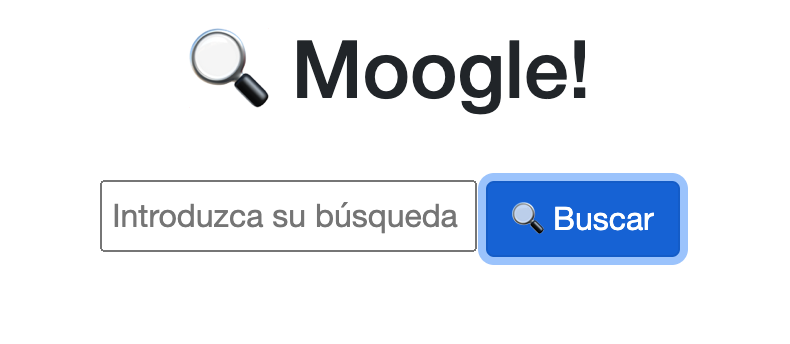
\includegraphics[width=10cm]{Pictures For Moogle!/Picture1.png}
\end{figure}

\begin{figure}[h]
    \center
    
\includegraphics[width=1cm]{Pictures For Moogle!/matcom.jpg}
    \label{fig:logo}
\end{figure}

\begin{abstract}
    Moogle! es una aplicacion cuyo proposito es buscar inteligentemente un texto en un conjunto de documentos. Es una aplicacion web, desarrollada con tecnologia .NET Core 6.0, especificamente usando Blazor como *framework* web para la interfaz grafica, y en el lenguaje CSharp.
\end{abstract}

\section {Introducción}\label{sec:intro}

Moogle! es una aplicación cuyo propósito es buscar inteligentemente un texto en un conjunto de documentos. Esta aplicación dada una query (texto a buscar) del usuario muestra en pantalla los documentos más importantes donde esa query aparece. La idea está en que la búsqueda sea lo más inteligente posible por eso no nos limitamos a solo mostrar exactamente el documento donde aparece exactamente esa query. Moogle implementa un algoritmo de búsqueda, muestra además sugerencias en caso de que la palabra introducida lo necesite, etc. Todo esto será explicado a detalle más adelante.

\section{Explicacion General}\label{sec: General}

Para poder obtener la relevancia de cada documento respecto a la búsqueda se ha utilizado la medida de recuperación de información de modelo vectorial y el valor TFIDF. Con este modelo vectorial vemos a los documentos y la Query como vectores que almacenaran sus valores TF-IDF respectivos. El TF-IDF (Term frequency – Inverse document frequency)no es más que la frecuencia de ocurrencia del término en la colección de documentos, la cual es una medida numérica que expresa cuán relevante es una palabra para un documento en una colección. Este valor aumenta proporcionalmente al número de veces que una palabra aparece en el documento, pero es compensada por la frecuencia de la palabra en la colección de documentos, lo que permite manejar el hecho de que algunas palabras son generalmente más comunes que otras. Con estos valores podemos verificar que tan parecidos son estos dos vectores mediante la Similitud del coseno. Esta es una medida de la similitud existente entre dos vectores en un espacio que posee un producto interior con el que se evalúa el valor del coseno del ángulo comprendido entre ellos. De esta manera mientras más cercano a 1 son los valores más cercanos a 0 es el ángulo existente entre los dos vectores y más parecidos son estos.

\section{Funcionalidad del Proyecto}\label{sec:General}

El proyecto comienza con la clase principal, la clase Moogle. Esta clase tiene un método Query que recibe a la query y devuelve los resultados de la búsqueda.
Primero debemos abstraernos y comenzar a ver cada documento como un vector. Necesitamos leer dado una dirección, cada documento y comenzar el proceso de leer el documento, tokenizarlo, obtener los valores TFIDF todo lo necesario para comenzar a resolver el problema inicial, devolver los mejores resultados de búsqueda posible. Lógicamente necesitamos información sobre el documento donde estamos para esto se implementó la Clase Document. Esta clase contiene toda la información necesaria sobre un documento en específico, su título, un método para hallar el vector TFIDF del documento, el texto del documento y todos los términos del documento guardados en un diccionario y donde se asocia ese término a la cantidad de veces que aparecen en el documento y además la primera posición donde fue encontrada dicha palabra en el documento (de gran utilidad para el snipet).

\begin{figure}[h]
    \center
    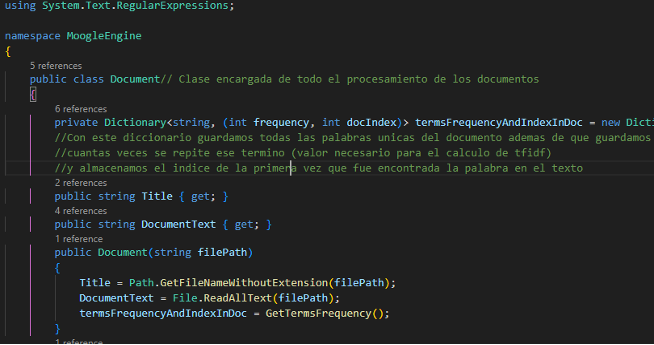
\includegraphics[width=10cm]{Pictures For Moogle!/Figure1.png}
    \caption{Muestra del codigo}
    \label{fig:logo}
\end{figure}

Importante destacar que a la hora de la tokenización del texto las palabras con tilde no se les elimina la tilde.

\begin{figure}[h]
    \center
    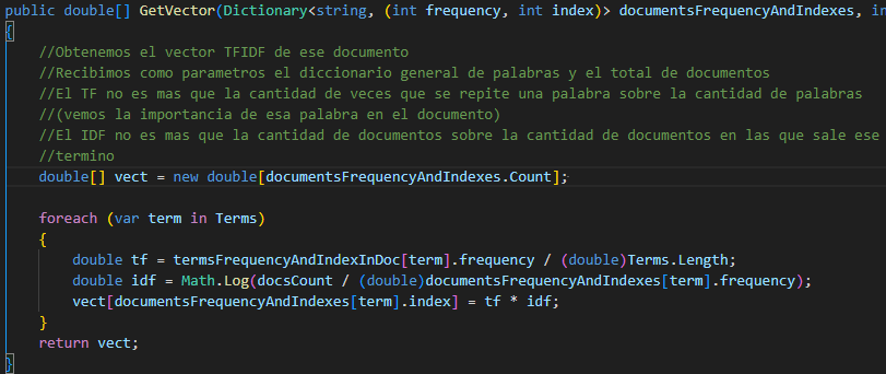
\includegraphics[width=10cm]{Pictures For Moogle!/Figure2.png}
    \caption{Vector TFIDF del documento}
    \label{fig:logo}
\end{figure}

Junto con esta clase tenemos la clase Query podemos decir que es hija de la clase documento. Para poder llevar la query a un vector debemos tratar a la query exactamente como trataríamos a un documento. Esta clase permite saber los términos de la query y su frecuencia en la misma además de cómo obtener su vector TFIDF. Igual que con la tokenizacion de los textos las palabras con tilde de la query no se les elimina la tilde.
La clase que ejecutara y trabajara todo es la clase UnrealEngine. Esta clase será la encargada de ejecutar todo lo necesario para la búsqueda. Esta clase posee un arreglo de Objetos documentos de la clase documento, es decir todos los documentos, además de todas las palabras generales del corpus dentro de un diccionario así asociamos a cada palabra (Key o llave) con la cantidad de documentos donde aparece la palabra  y un índice asociado para así mantener un control sobre las palabras y proceder a ubicarlas en la matriz TFIDF más cómodamente. 

\begin{figure}[h]
    \center
    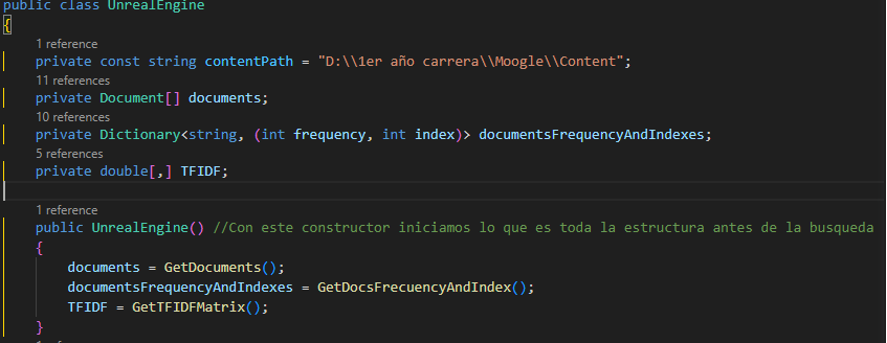
\includegraphics[width=10cm]{Pictures For Moogle!/Figure3.png}
    \caption{Class UnrealEngine}
    \label{fig:logo}
\end{figure}

Este es el proceso de obtención de palabras generales del corpus es sencillo  GetDocsFrecuencyAndIndex () en términos generales recorre cada documento y por cada documento recorre sus términos estos los va almacenando en el diccionario en caso de que ya tenga esa palabra le suma uno a su frecuencia y mantiene su índice en caso contrario agrega 1 a su frecuencia y el índice asociado es el tamaño que posea el diccionario hasta ese momento.
Una vez obtenido todas las palabras del corpus y todos los vectores TFIDF necesarios para construir la matriz podemos tener el espacio creado para próximamente realizar las búsquedas.

Proceso de Obtención de la matriz.

\begin{figure}[h]
    \center
    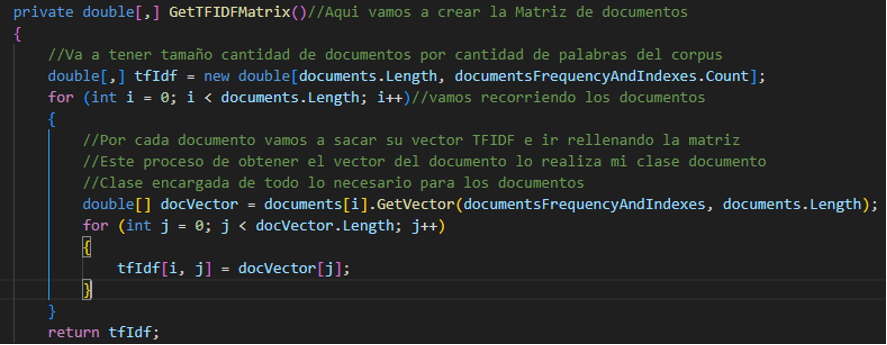
\includegraphics[width=10cm]{Pictures For Moogle!/Figure4.png}
    \caption{Obtención de la matriz}
    \label{fig:logo}
\end{figure}

Ya una vez con la query tratada como un vector de TFIDF y todos los documentos almacenados en una matriz que guarda el TFIDF de cada vector documento solo queda pasar a la acción y comenzar la búsqueda. Una vez se introduce la búsqueda esta pasa a un vector tamaño n donde pasamos a realizar la antes comentada similitud del coseno entre ese vector de la query y cada uno de los vectores documentos de la matriz. Una vez terminado el proceso organizamos los score y devolvemos los mejores documentos para el usuario.
Es importante recalcar que una vez construido un objeto de tipo UnrealEngine comenzara a cargarse toda la base de datos una y solo una vez, luego de esto estamos listos para comenzar la búsqueda.

\section{Implementaciones Extras:}\label{sec:Extras}

El programa es capaz de devolver además porciones de los textos más relevantes donde aparezca la query deseada. Relativamente sencillo al ya tener las posiciones donde aparece cada termino en el texto. Para esto revisamos cual termino de nuestra query es el más relevante y buscamos su índice en el texto y solo queda obtener tantos  caracteres a la izquierda y derecha se desee y se devuelve dicho fragmento.
También tiene implementada una funcionalidad para dar sugerencias en caso de que algún término de la query no aparezca en el corpus se le recomendara al usuario la palabra más similar entre todas las palabras del corpus este proceso se hace mediante la distancia de levenshtein. Esta distancia es el mínimo número de operaciones que se deben hacer para convertir una palabra en otra se entiende por operaciones las siguientes tres, Insertar una palabra, Eliminar una palabra y la Sustitución de una palabra.
Como un extra en la parte visual podemos dar clic en la sugerencia dada y comenzara una nueva búsqueda en función de la sugerencia.


\begin{figure}[h]
    \center
    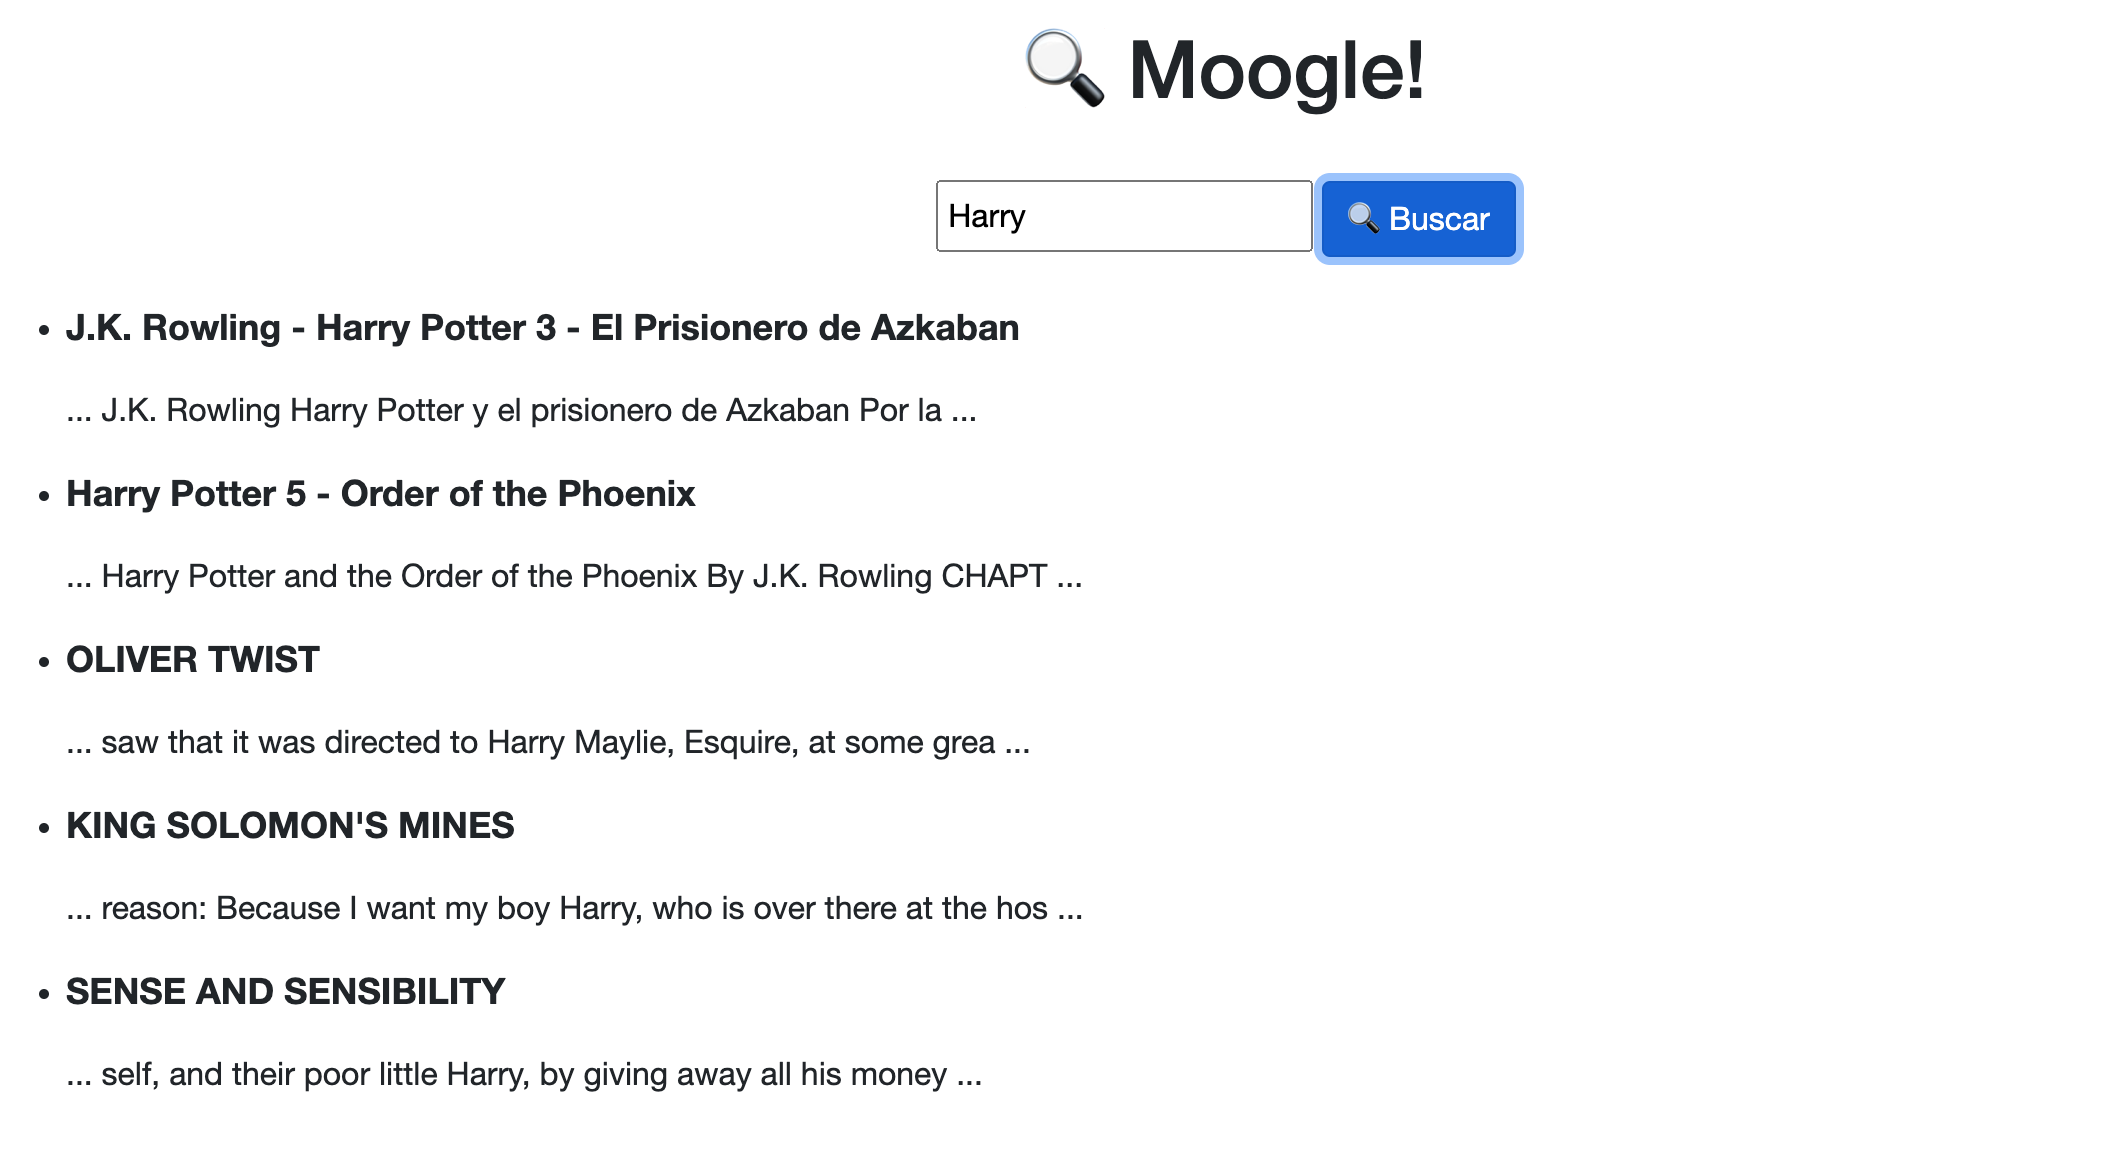
\includegraphics[width=10cm]{Pictures For Moogle!/Picture2.png}
    \caption{Busqueda realizada con exito y con un fragmento del texto donde la palabra buscada aparece}
    \label{fig:logo}
\end{figure}

\begin{figure}[h]
    \center
    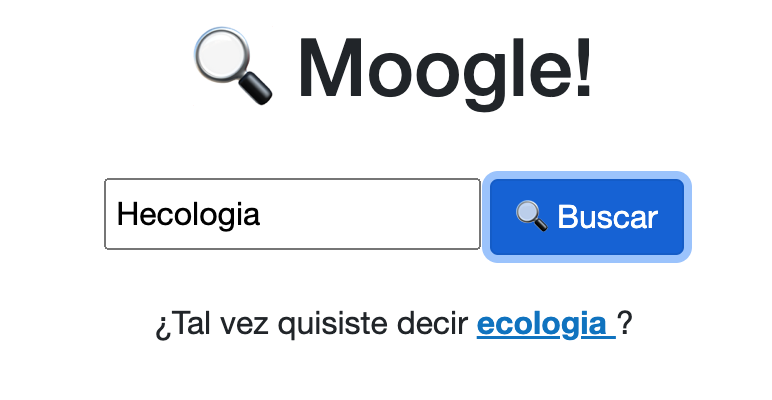
\includegraphics[width=10cm]{Pictures For Moogle!/Picture3.png}
    \caption{Ejemplo de como el se ofrece la sugerencia (notese el enlace que puede se tocado en la sugerencia para iniciar una nueva busqueda)}
    \label{fig:logo}
\end{figure}

\begin{figure}[h]
    \center
    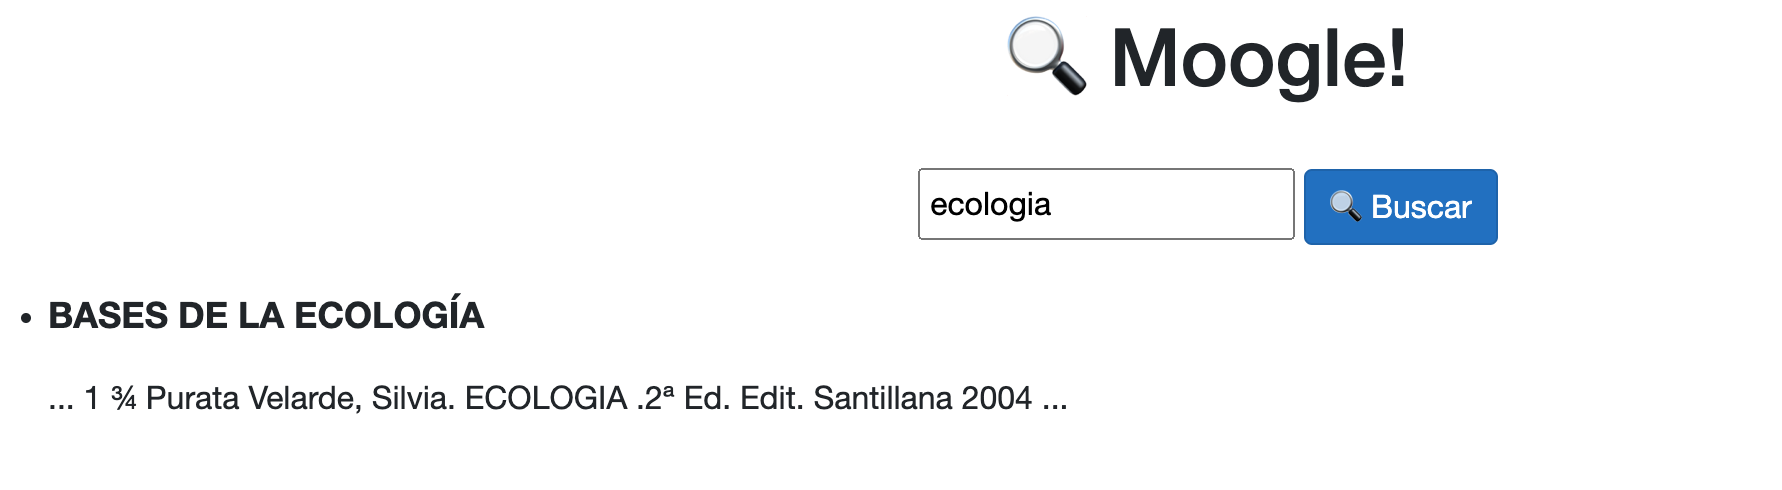
\includegraphics[width=15cm]{Pictures For Moogle!/Picture4.png}
    \caption{Nueva busqueda con la sugerencia}
\end{figure}
\tableofcontents
\end{document}